% \documentclass{book}

\documentclass[12pt]{article}
\usepackage[pdfborder={0 0 0.5 [3 2]}]{hyperref}%
\usepackage[left=1in,right=1in,top=1in,bottom=1in]{geometry}%
\usepackage[shortalphabetic]{amsrefs}%
\usepackage{amsmath}
\usepackage{enumerate}
\usepackage{enumitem}
\usepackage{amssymb}                
\usepackage{amsmath}                
\usepackage{amsfonts}
\usepackage{amsthm}
\usepackage{bbm}
\usepackage[table,xcdraw]{xcolor}
\usepackage{tikz}
\usepackage{float}
\usepackage{booktabs}
\usepackage{svg}
\usepackage{mathtools}
\usepackage{cool}
\usepackage{url}
\usepackage{graphicx,epsfig}
\usepackage{makecell}
\usepackage{array}

\def\noi{\noindent}
\def\T{{\mathbb T}}
\def\R{{\mathbb R}}
\def\N{{\mathbb N}}
\def\C{{\mathbb C}}
\def\Z{{\mathbb Z}}
\def\P{{\mathbb P}}
\def\E{{\mathbb E}}
\def\Q{\mathbb{Q}}
\def\ind{{\mathbb I}}

\graphicspath{ {images5/} }

\begin{document}
\section*{12 Feb 2017}
Further work with the 5th order KdV equation led me to believe that we were reaching the level of machine precision with our numerical methods, i.e. the eigenvalues we got were so tiny that it was hard to tell if they were meaningful or not. On recommendation, I decided to try a different (but related) equation: a two-parameter, 5th order model for shallow water waves, which I will call the Shallow Water Equation. This is Equation 1.1 in Chapneys and Groves (1997) or Equation 6.16-6.17 in Sandstede (2015).

\subsubsection*{Background}

\[
u_t + \partial _x\left( \frac{2}{15}u_{xxxx} - b u_{xx} + \frac{3}{2}u^2 + \frac{1}{2}u_x^2 + u u_{xx} \right) = 0
\]
Traveling waves $u = u(x + ct)$ satisfy the 4th order equation (keeping the variable as x):
\[
 \frac{2}{15}u_{xxxx} - b u_{xx} + c u + \frac{3}{2}u^2 + \frac{1}{2}u_x^2 + u u_{xx} = 0
\]
From Chapneys and Groves (1997), this has an explicit localized solution:
\[
u_*(x) = 3\left( b + \frac{1}{2} \right) \sech^2 \left( \sqrt{3(2 b + 1)} \frac{x}{2} \right)
\]
which is valid for $b > -1/2$ and $c = c_*(b)$, where
\[
c_*(b) = \frac{3}{5}(2b+1)(b-2)
\]
Linearizing this around the a solution $u_*$, we obtain the Jacobian:
\[
J = \frac{2}{15} \partial_x^4 + (u_* - b)\partial_x^2 + u_*' \partial_x + (c + 3 u_* + u_*'')
\]
If we linearize about the solution $u_* = 0$, we get the eigenvalue relation:
\[
\frac{2}{15}\lambda^4 - b\lambda^2 _ c = 0
\]
Note that for $c = c_*(b)$, all eigenvalues $\lambda$ are real, and there are no oscillations in the solution $u_*(x)$, which is a simple pulse which decays exponentially on both sides.\\

For the 5th-order equation, the Jacobian is 
\[
J = \frac{2}{15} \partial_x^5 + (u_* - b)\partial_x^3 + 2 u_*' \partial_x^2 + (3 u_* + 2u_*'')\partial_x + (c + 3 u_*' + u_*''')
\]

The procedure is as follows:
\begin{enumerate}
	\item Choose parameter $b$ first. Sanstede (2015) suggests that to have multipulses we need to choose $b > 2$, so we initially take $b = 2.5$ (admittedly an arbitrary choice). Interestingly, Chapneys and Groves (1997) show multipulses in many different parameter regimes, including $b = -0.5, c = 1$ (figure 3, p 210); and $b = 0.5, c = 2$ (figure 22, p. 224). These may be work exploring at some point.
	\item Start with known solution $u_*(x)$ with $c = c_*(2.5) = 1.8$.
	\item Use Fourier spectral methods with periodic BCs on interval $[-L, L]$. There is a tradeoff between making the domain large enough so the pulses do not interact with the (periodic) boundary and small enough so that the code can run on my computer. Large numbers of grid points, in particular, are wasteful since the solution is zero for most of the domain. It might be interesting to try an adaptive mesh at some point. For now, we chose $L = 20$ and $N = 2048$. The Fourier differentiation operator does introduce small oscillations at the base of the pulse (just try $D*u_*$), but for $N = 2048$ this is manageable. I tried filtering briefly, but it made things worse.
	\item Use continuation to increase $c$ so that we have complex eigenvalues $\lambda$ for the linearization about $u_* = 0$. Resulting pulse has tail oscillations, as expected, whose angular frequency is given (roughly) by the 
	\item Construct double pulses from the single pulse by gluing together the single pulses at the appropriate places. These turn out to be:
		\begin{enumerate}
			\item First min (visible dip below baseline)
			\item Halfway between first min and first max
			\item First max (visible bump above baseline)
			\item Halfway between first max and second min
			\item Second min (it's there, but you can't see it)
			\item etc
		\end{enumerate}
	Note that we are constructing pulses at halfway points between the mins and maxes. THIS IS NEW. I got this from Chapneys and Groves, figure 22. Graph (b) joins at the first min of (a). Graph (d) joins at the first max of (a). I had never seen graph (c) before, but it looks like the pulses are spaced at integer multiples of a constant, so halfway between seems reasonable.
\end{enumerate}

From previous numerical experiments, all our double pulses had a pair of real eigenvalues $\lambda, -\lambda$. We never got the expected pattern where this alternated with either a quadruplet or with complex eigenvalues. My hypothesis here is that our previous results were correct, but that were were MISSING HALF OF THE DOUBLE PULSES. The missing ones are constructed at the half-way points. Let's try this and see what happens.

\subsubsection*{Initial trial}
Using a fixed $b = 2.5$, we ran the continuation code until $c =  238.7352
$. This was likely massive overkill, but larger $c$ makes the eigenvalues larger (less risk of numerical error) and makes the pulses closer to the center (higher frequency oscillations), making the domain size matter less. It also makes the max/mins more prominent. Let's look at the graphs and the eigenvalues of the linearization about the solution. These are the eigenvalues of the 5th order ODE (not the integrated version). If we have real eigenvalues, eigenfunctions are also shown.

\begin{enumerate}
	\item Single pulse
	\begin{figure}[H]
	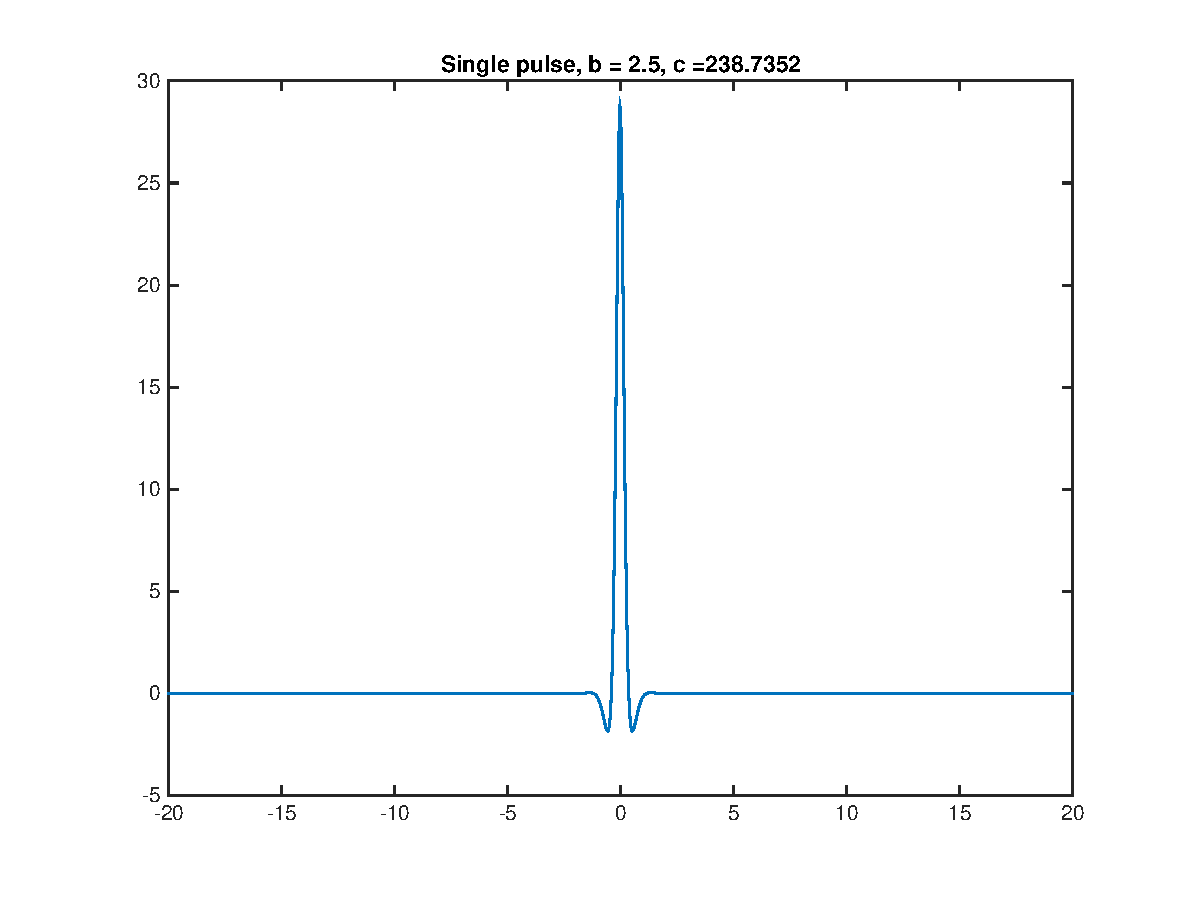
\includegraphics[width=8.5cm]{1single.eps}
	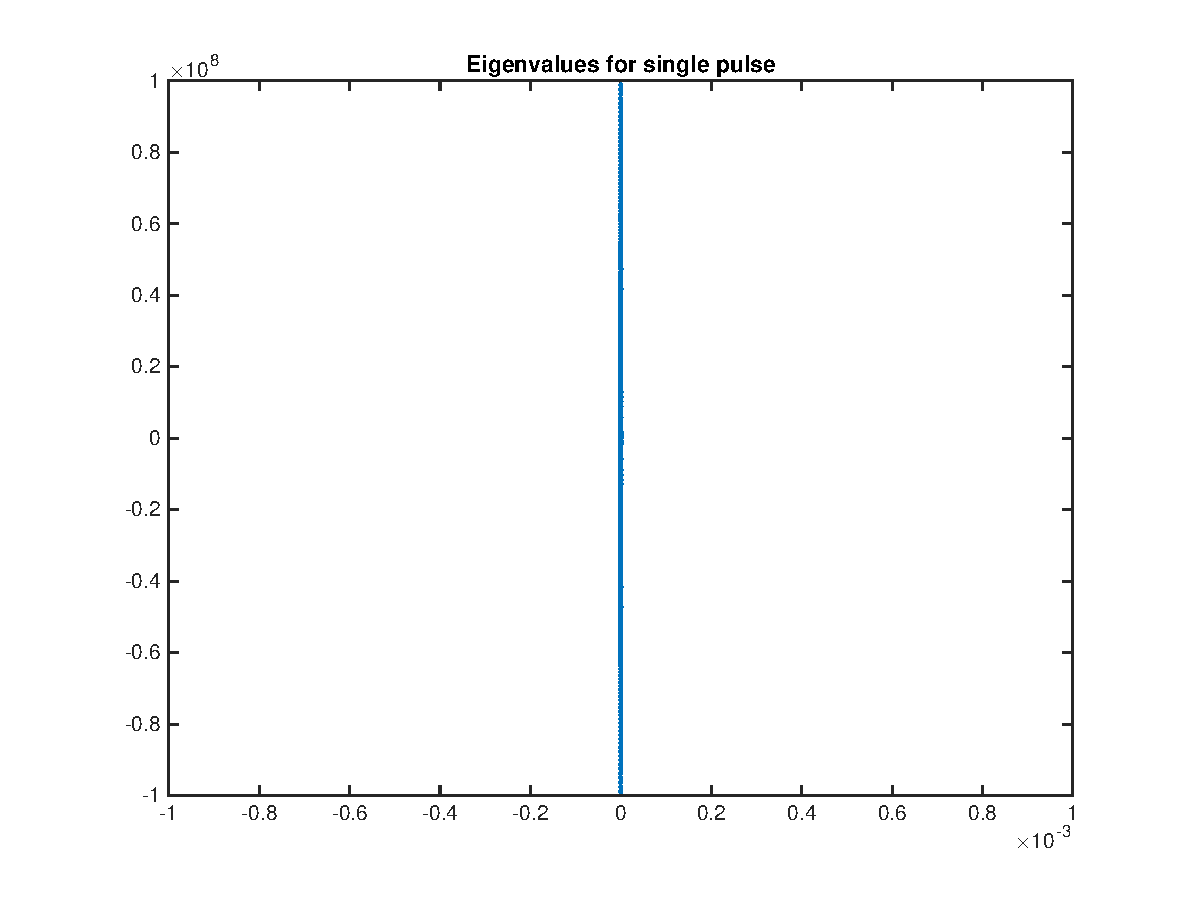
\includegraphics[width=8.5cm]{1singleeig.eps}
	\end{figure}
	

	\item Double pulse 1: joined at 1st min
	\begin{figure}[H]
	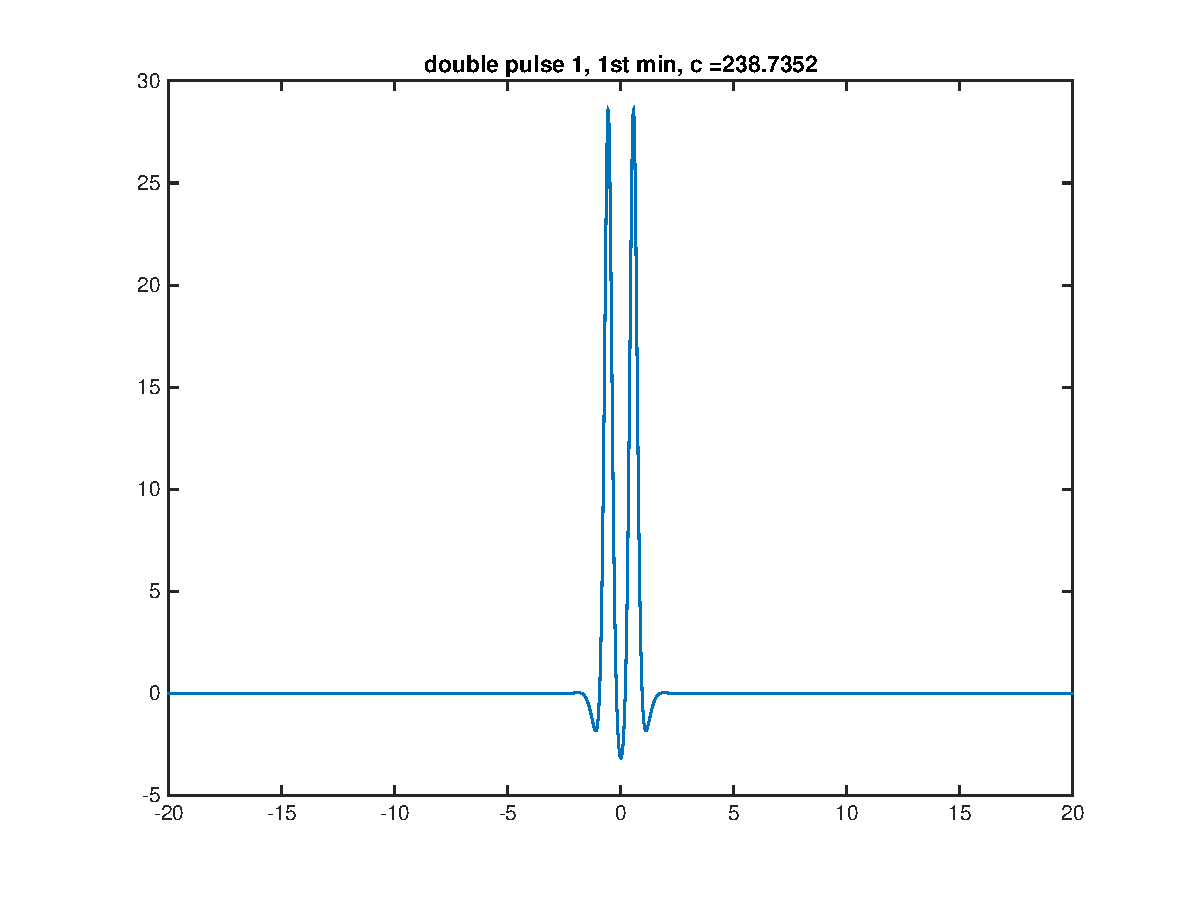
\includegraphics[width=8.5cm]{1double1.eps}
	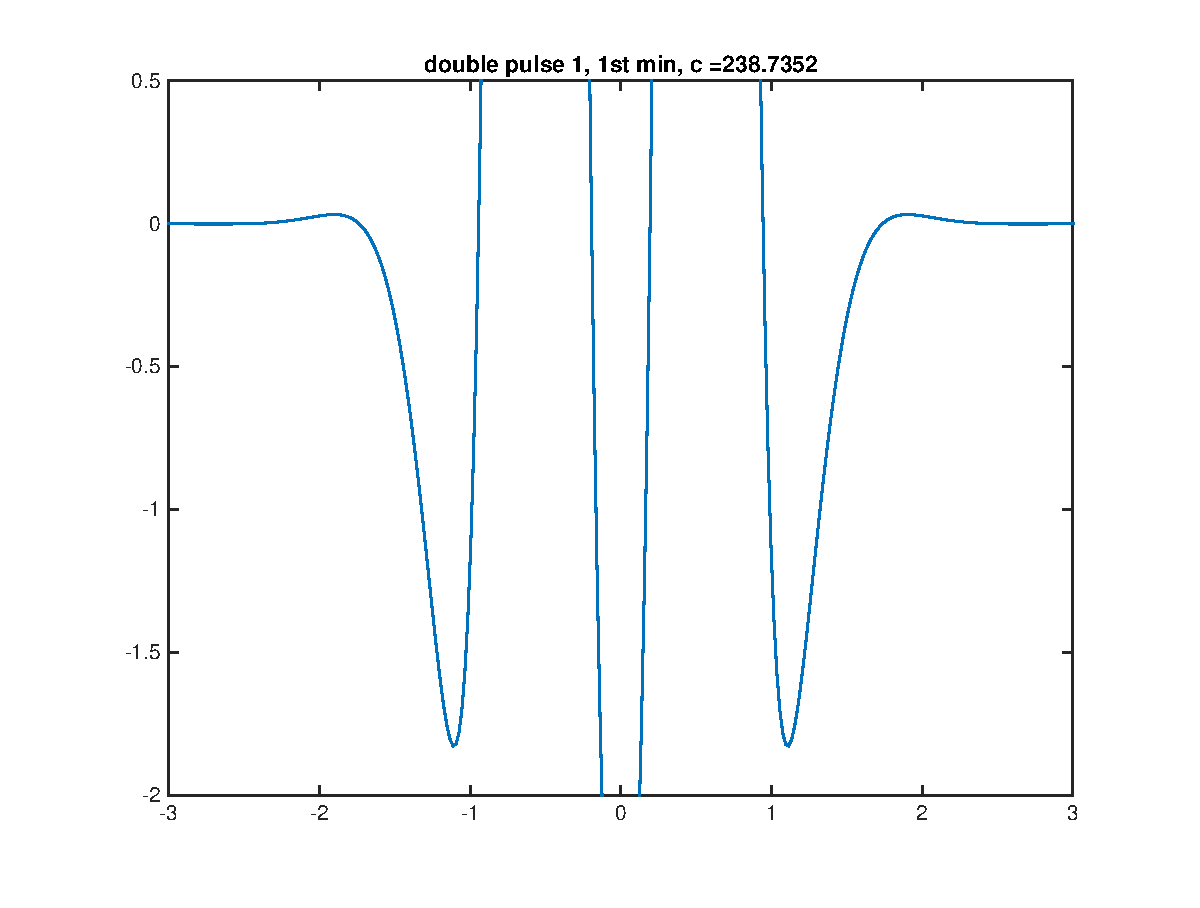
\includegraphics[width=8.5cm]{1double1zoom.eps}
	\end{figure}
	\begin{figure}[H]
	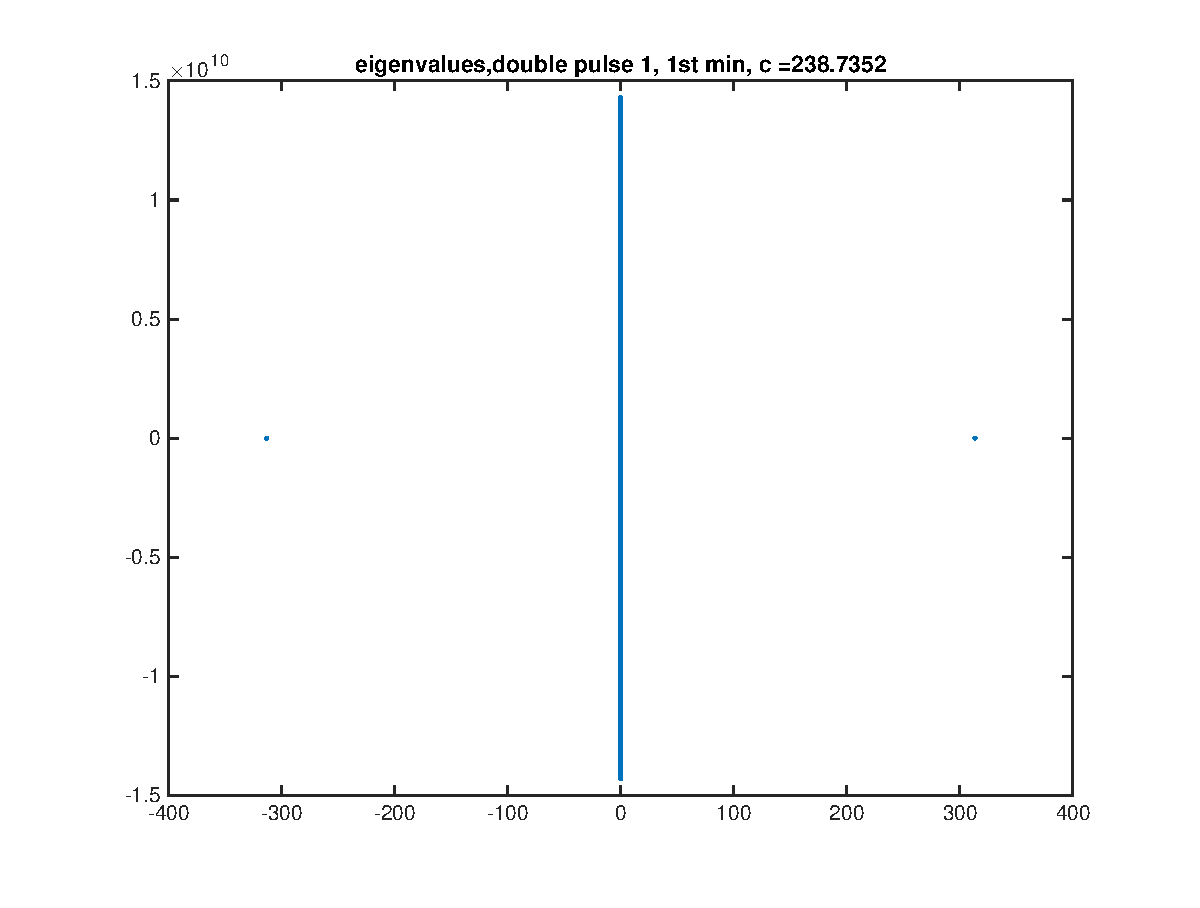
\includegraphics[width=8.5cm]{1double1eig.eps}
	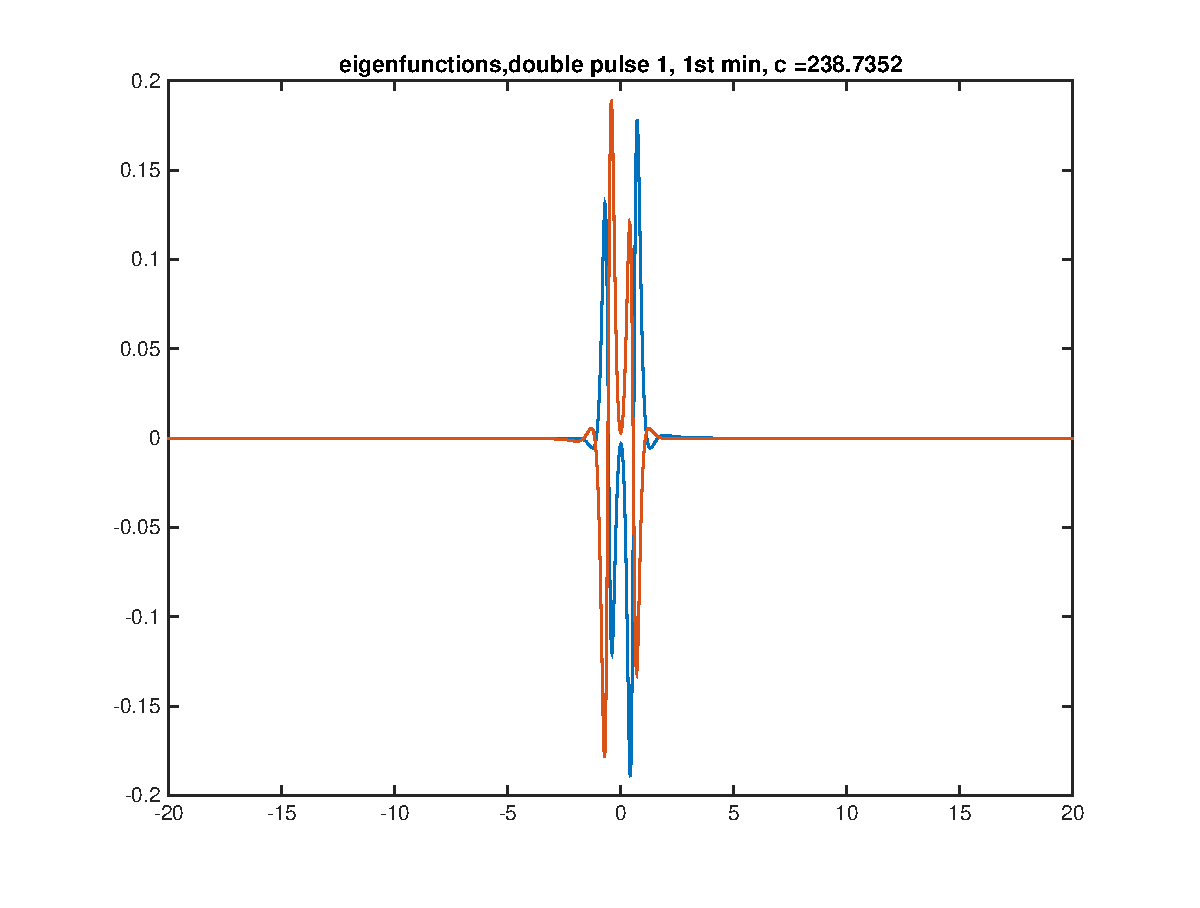
\includegraphics[width=8.5cm]{1double1eigfn.eps}
	\end{figure}

	\item Double pulse 2: joined between 1st min and 1st max
	\begin{figure}[H]
	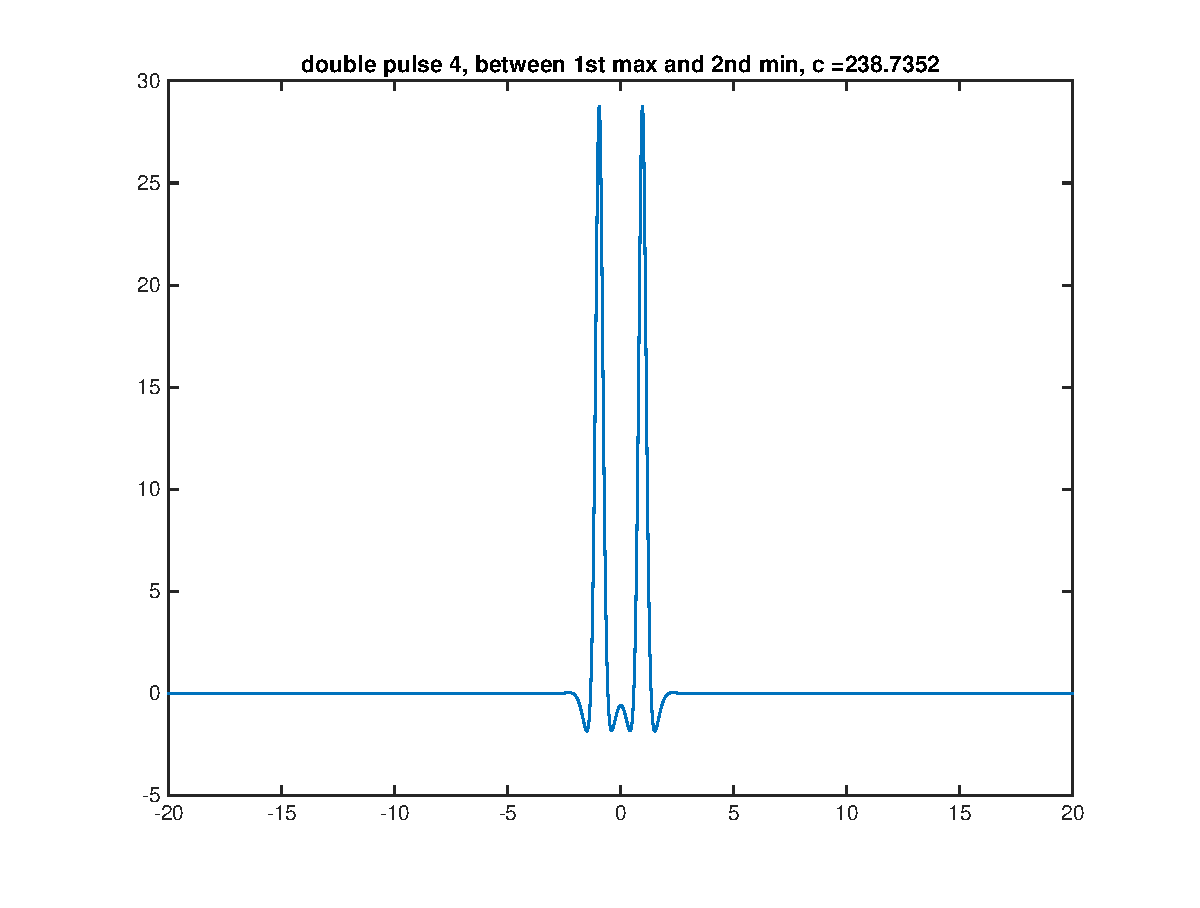
\includegraphics[width=8.5cm]{1double2.eps}
	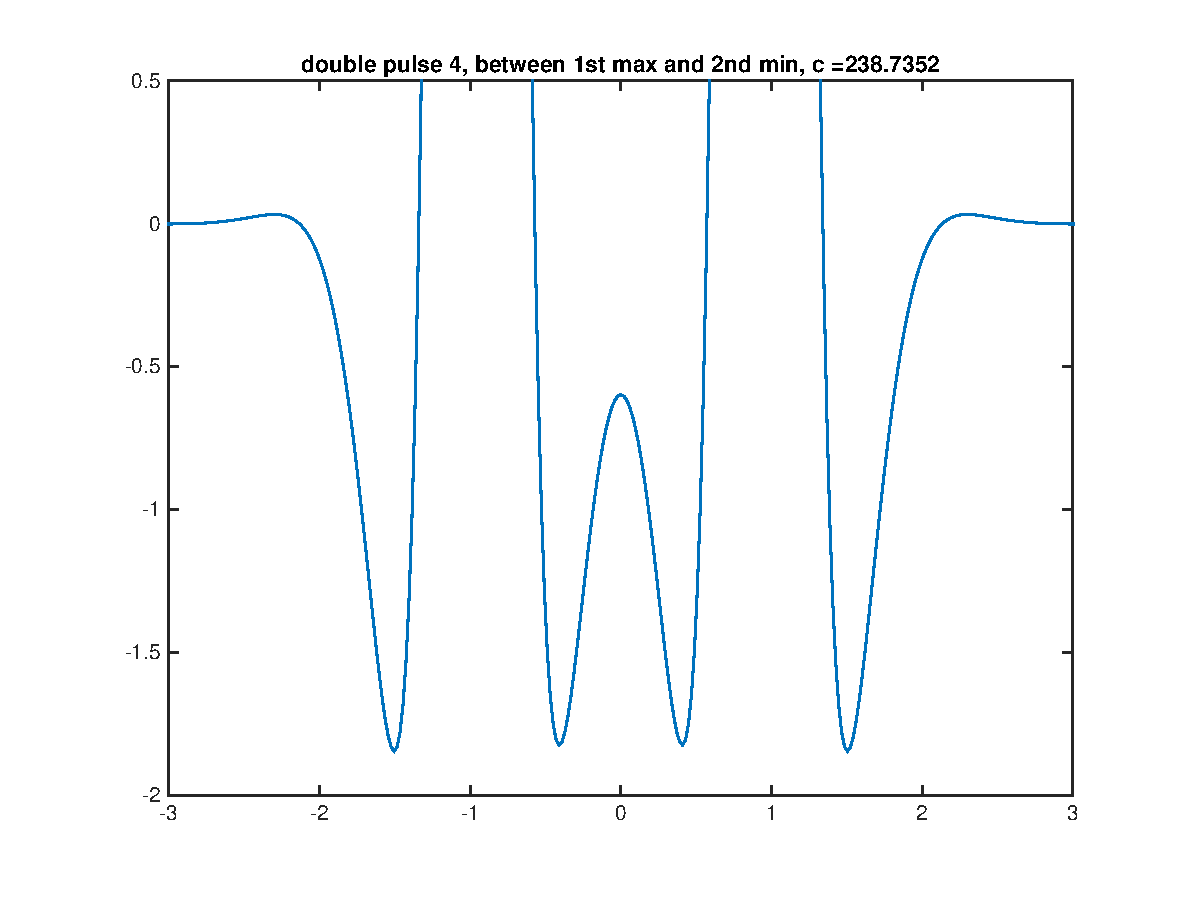
\includegraphics[width=8.5cm]{1double2zoom.eps}
	\end{figure}
	\begin{figure}[H]
	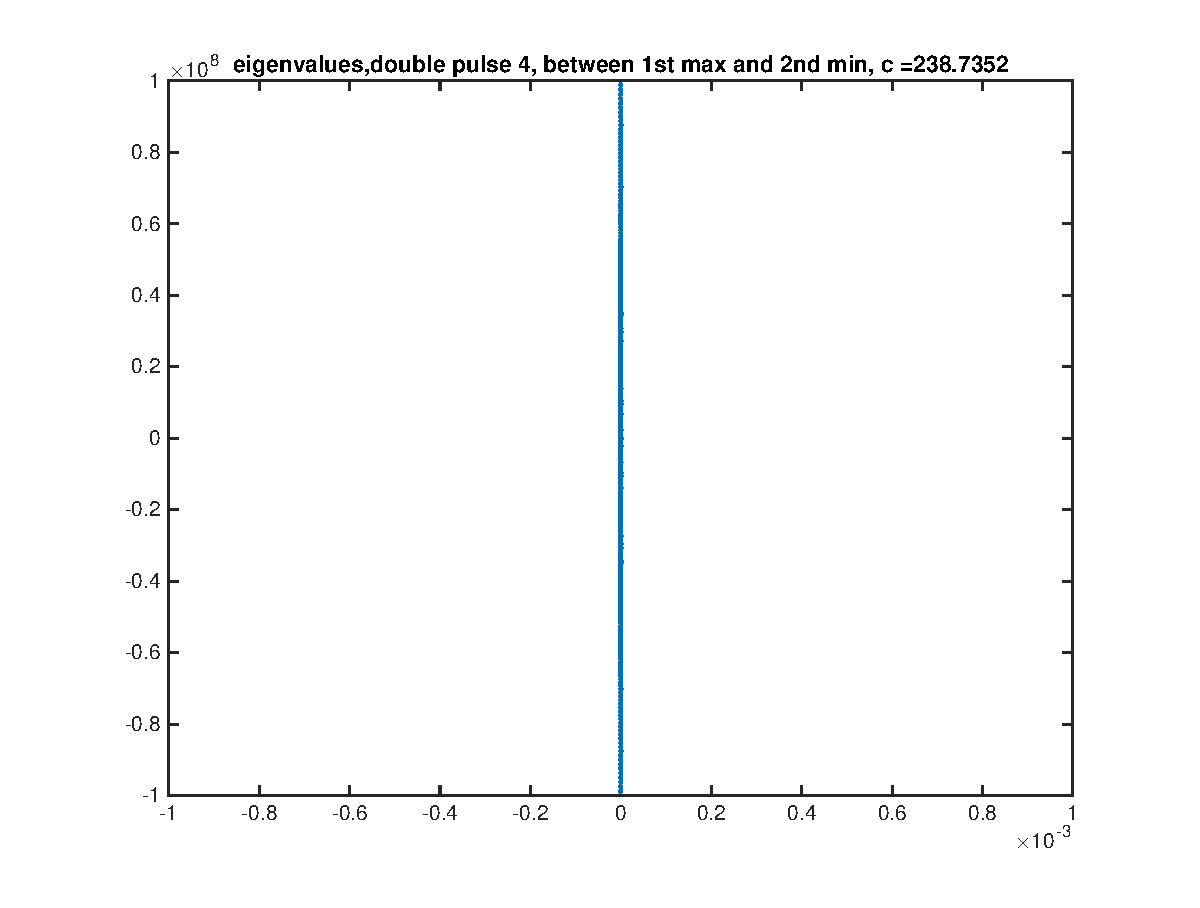
\includegraphics[width=8.5cm]{1double2eig.eps}
	\end{figure}

	\item Double pulse 3: joined at 1st max
	\begin{figure}[H]
	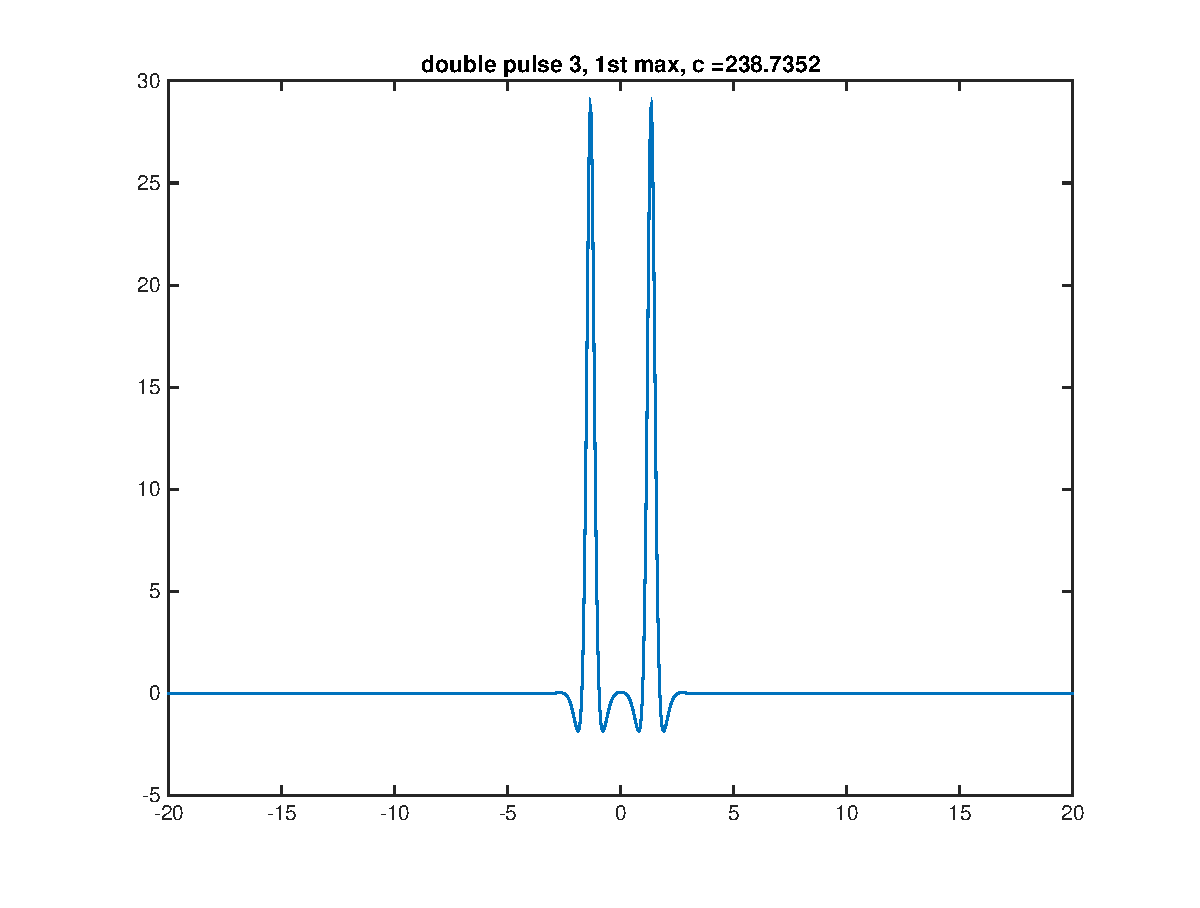
\includegraphics[width=8.5cm]{1double3.eps}
	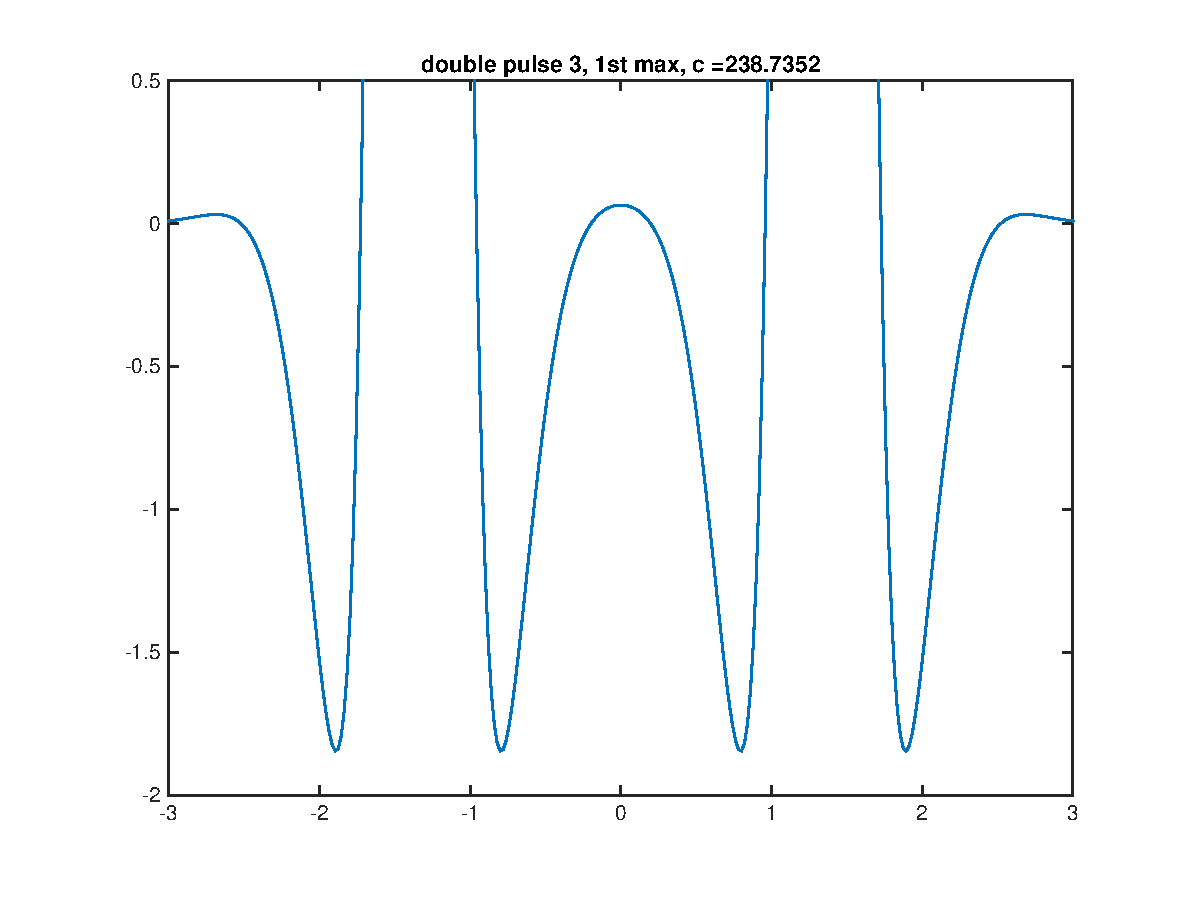
\includegraphics[width=8.5cm]{1double3zoom.eps}
	\end{figure}
	\begin{figure}[H]
	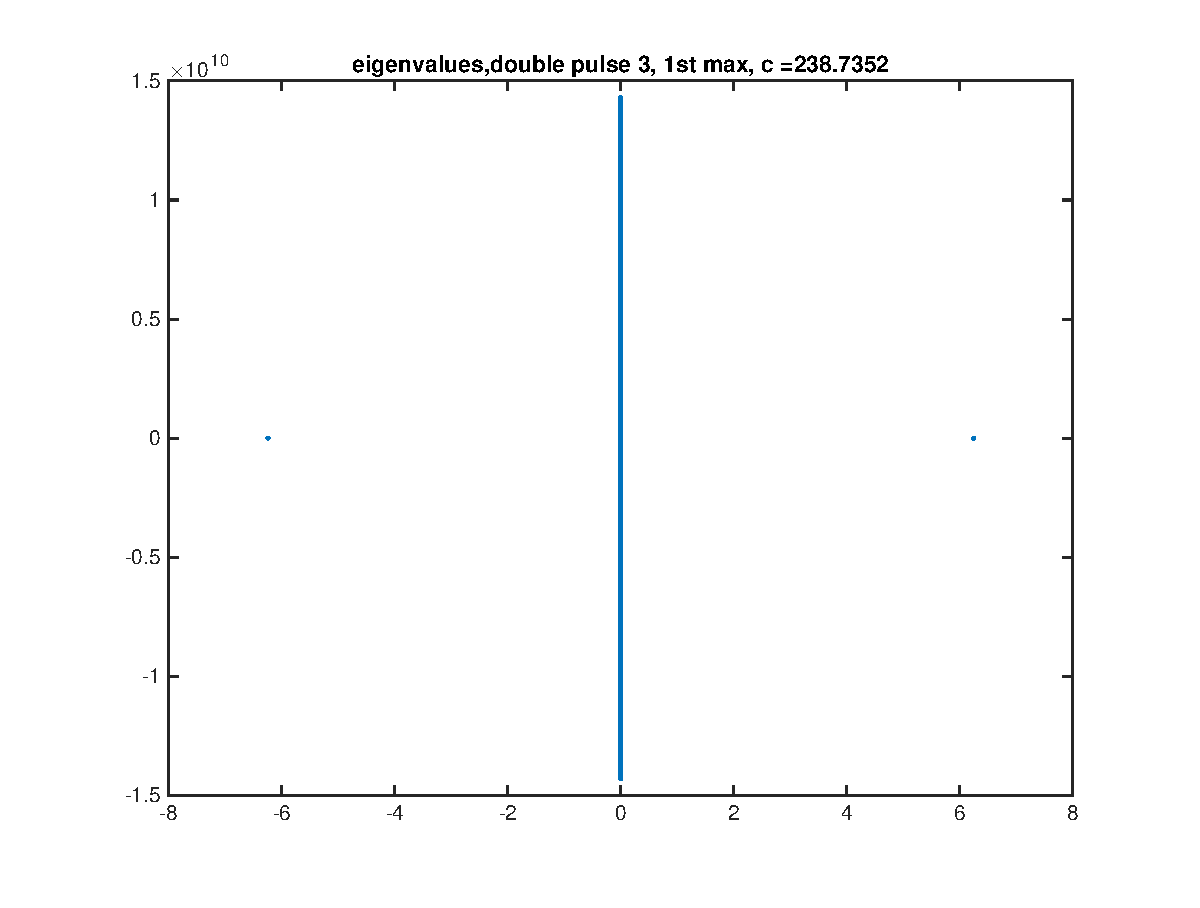
\includegraphics[width=8.5cm]{1double3eig.eps}
	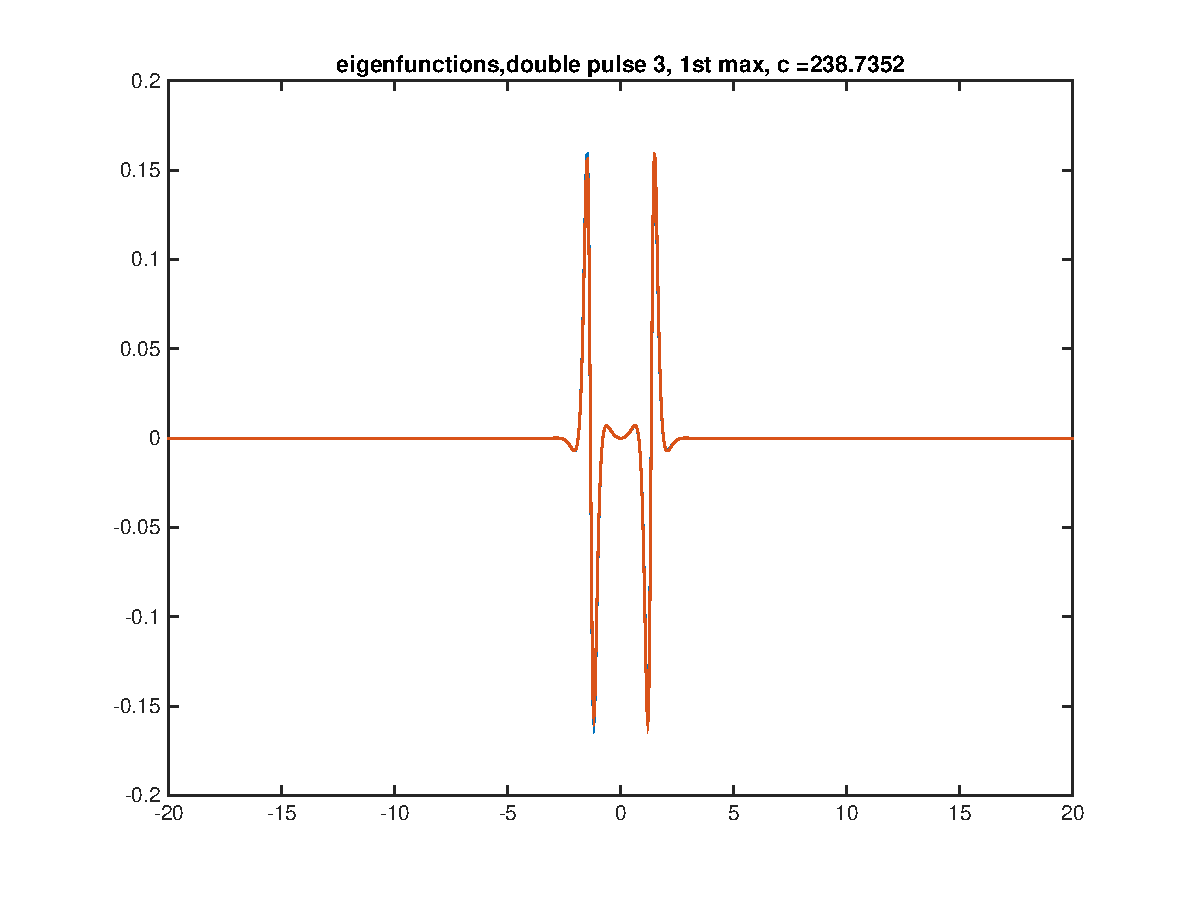
\includegraphics[width=8.5cm]{1double3eigfn.eps}
	\end{figure}

	\item Double pulse 4: joined between 1st max and 2nd min
	\begin{figure}[H]
	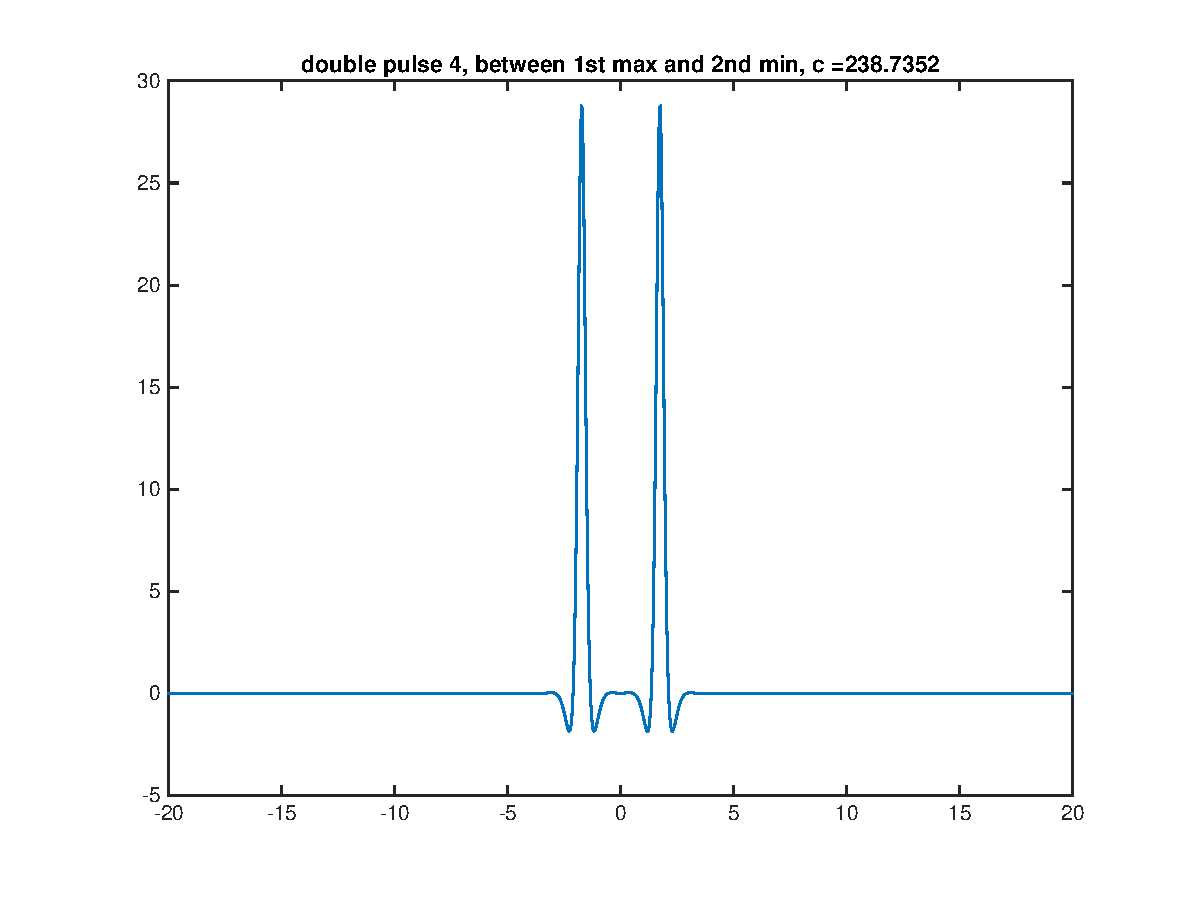
\includegraphics[width=8.5cm]{1double4.eps}
	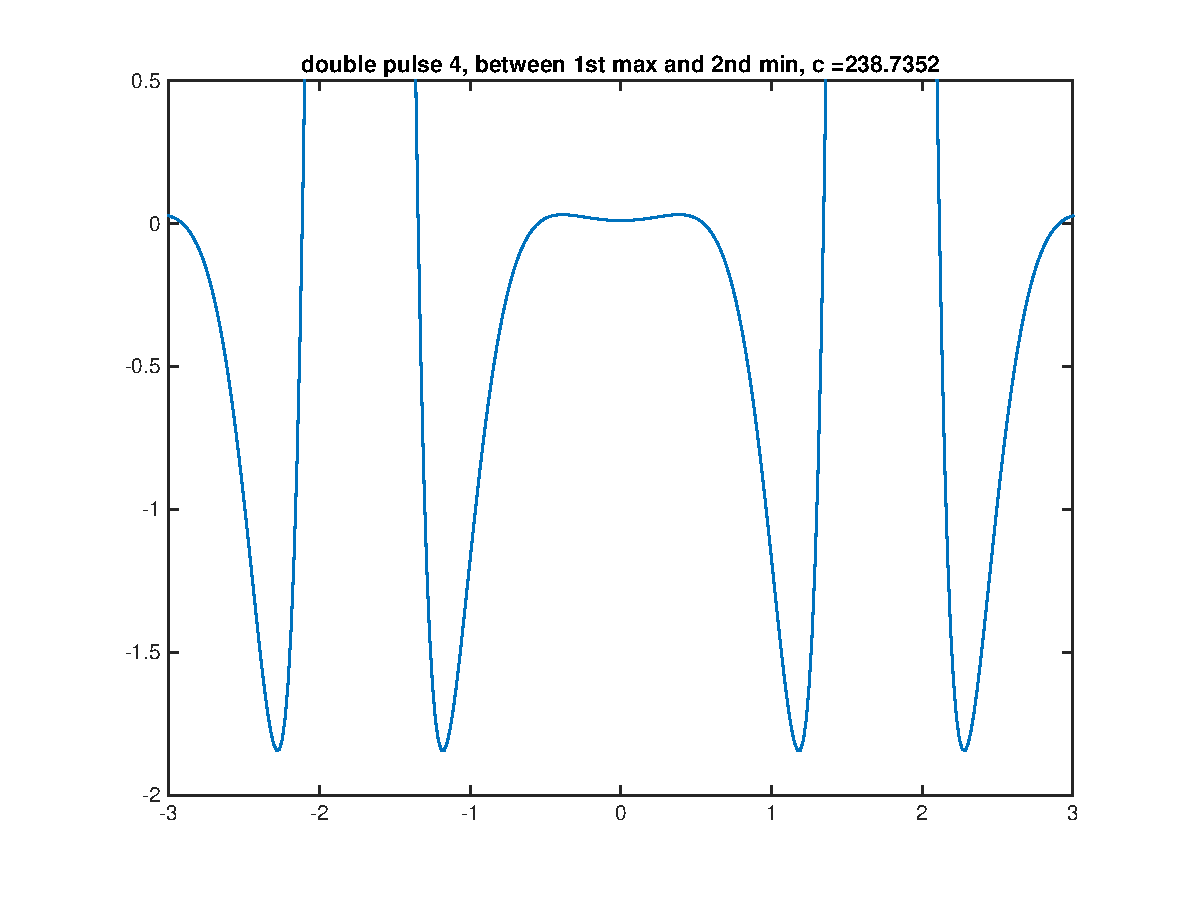
\includegraphics[width=8.5cm]{1double4zoom.eps}
	\end{figure}
	\begin{figure}[H]
	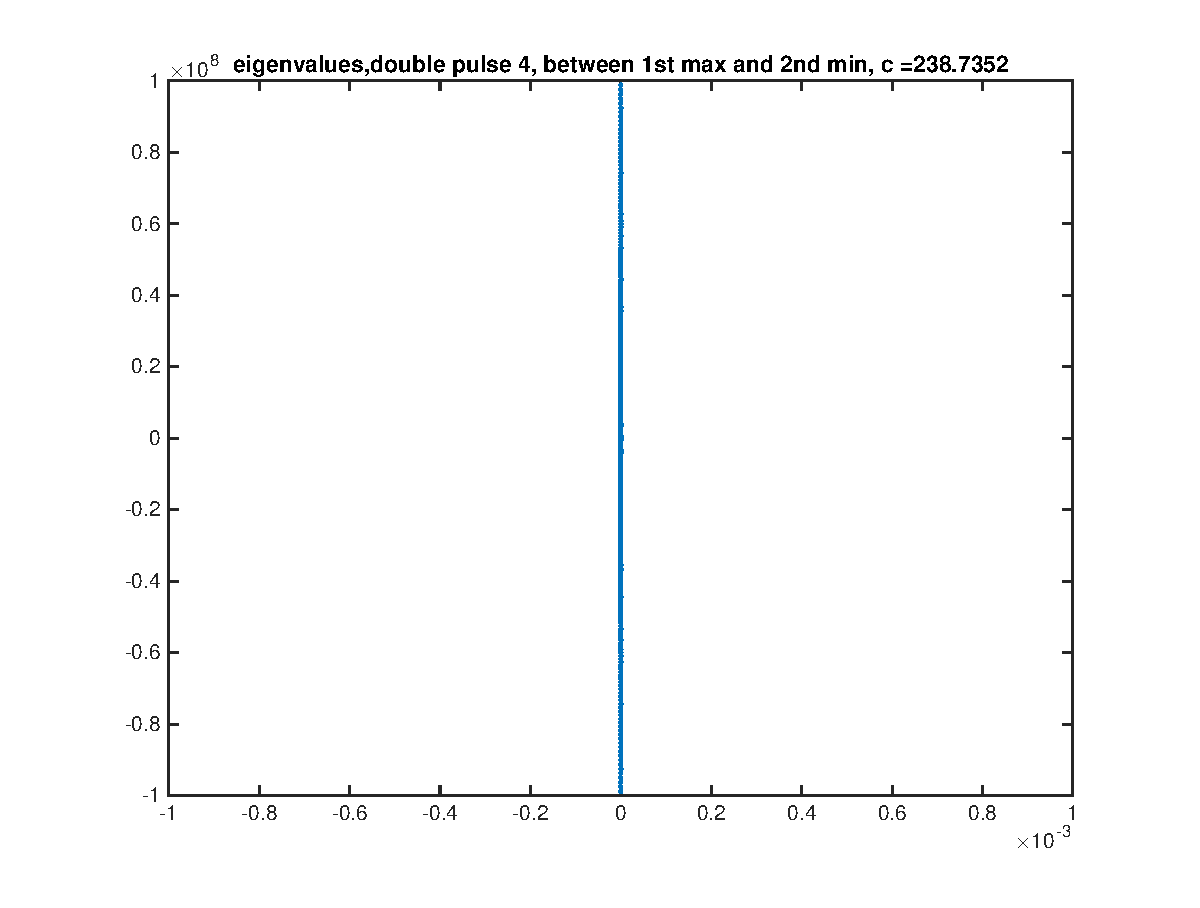
\includegraphics[width=8.5cm]{1double4eig.eps}
	\end{figure}

\end{enumerate}

So we have two real eigenvalues $\lambda, -\lambda$ alternating with no real eigenvalues, so this looks good (I think.) For double pulses 2 and 4, should have a pair of pure imaginary, complex conjugate eigenvalues, but these are hiding in the essential spectrum and I'm not sure how to find them.\\

We can check this by looking at the eigenvalues of the integrated operator. For double pulses, we should have a pair near 0 and a pair of negative eigenvalues. This is indeed the case. The table below just shows these eigenvalues. As expected, the paired eigenvalue near 0switches sides each time, so this is also good.

\begin{figure}[H]
\begin{tabular}{ll|ll|ll}
Pulse  &         & Eigenvalue near 0  & Paired eigenvalue & Other eigenvalue  & Paired eigenvalue \\ \hline
Single &         & 1.7053e-12         &                   & -672.5226         &                   \\
D1     & min     & -8.3423e-10        & 5.6405            & -664.7391         & -664.1654       \\
D2     & between & 7.4522e-10         & -0.10438          & -672.6659         & -672.6513       \\
D3     & min     & -8.4333e-10        & 0.0020            & -672.5199         & -672.5199       \\
D4     & between & -1.8552e-08        & -3.9913e-05       & -672.5227         & -672.5227       \\
\end{tabular}
\end{figure}
For pulses D3 and D4, the negative eigenvalues are not identical (i.e. they come in a pair), but the gap is too small to see in the table (they are separated by about 1e-7). It also appears that the double pulse eigenvalue gap is closing to 0 and each pair approaches the single eigenvalue for the single pulse. This makes sense, as if the pulses are far enough away, they don't really interact, so what we have is not that different from a single pulse.

\subsubsection*{Back to KdV}
Since this looks hopeful, does this work for the 5th order KdV equation. We repeat the above with the 5th order KdV using Fourier spectral methods with $N = 1024$ and $L = 50$. Speed is $c = 1.5672$. We only do the first three double pulses, because we then run into numerical instability. It looks like the same pattern holds, which is good. We could likely extend this to further double pulses if we used more grid points, a higher $c$, or a longer domain. Interestingly, in this case we can also get a ``Double Pulse 0'', which we get by joining the pulses half way between the origin and the first min. It follows the same eigenvalue pattern. It is possible that we could get one of these for the Shallow Water equation, but we'd want to try that where the pulse is wider.

\begin{enumerate}
	\item Single pulse
	\begin{figure}[H]
	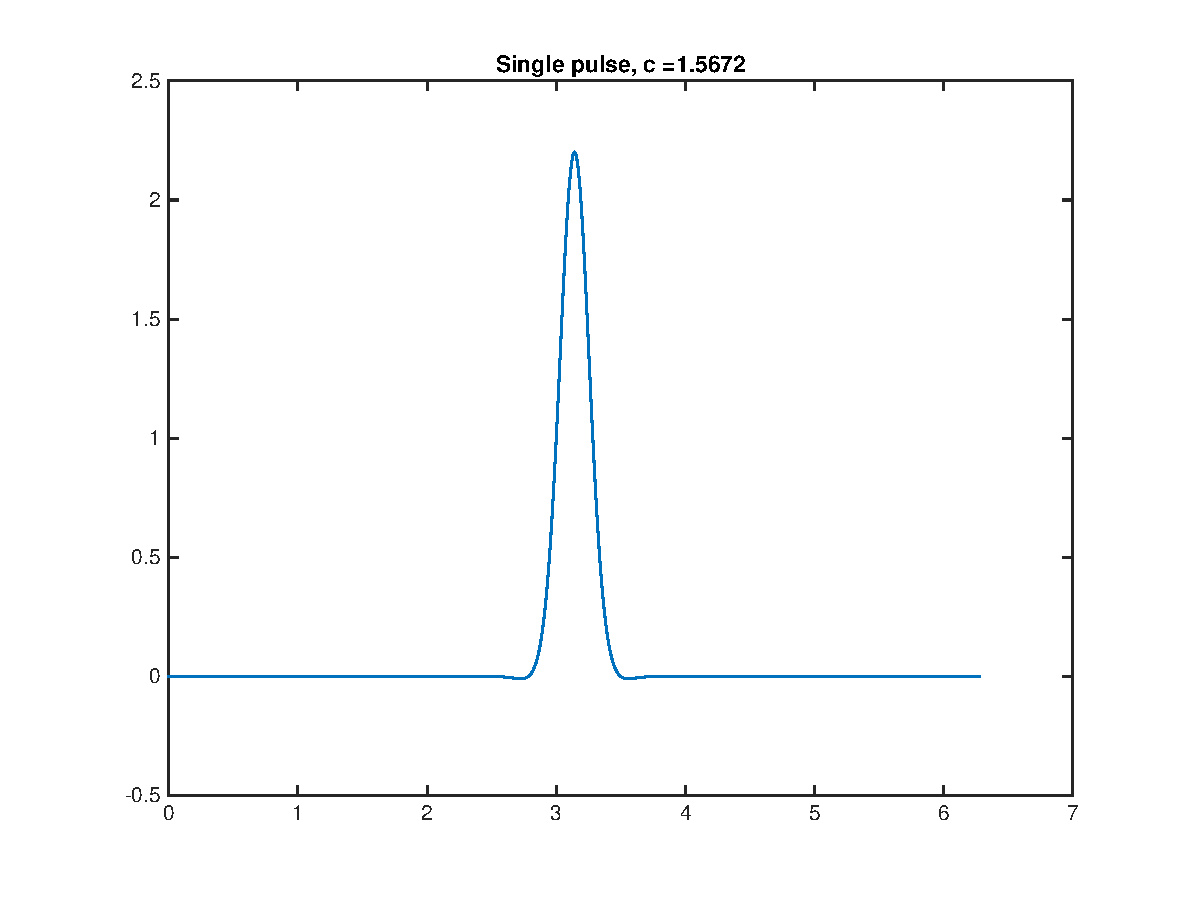
\includegraphics[width=8.5cm]{KdVsingle.eps}
	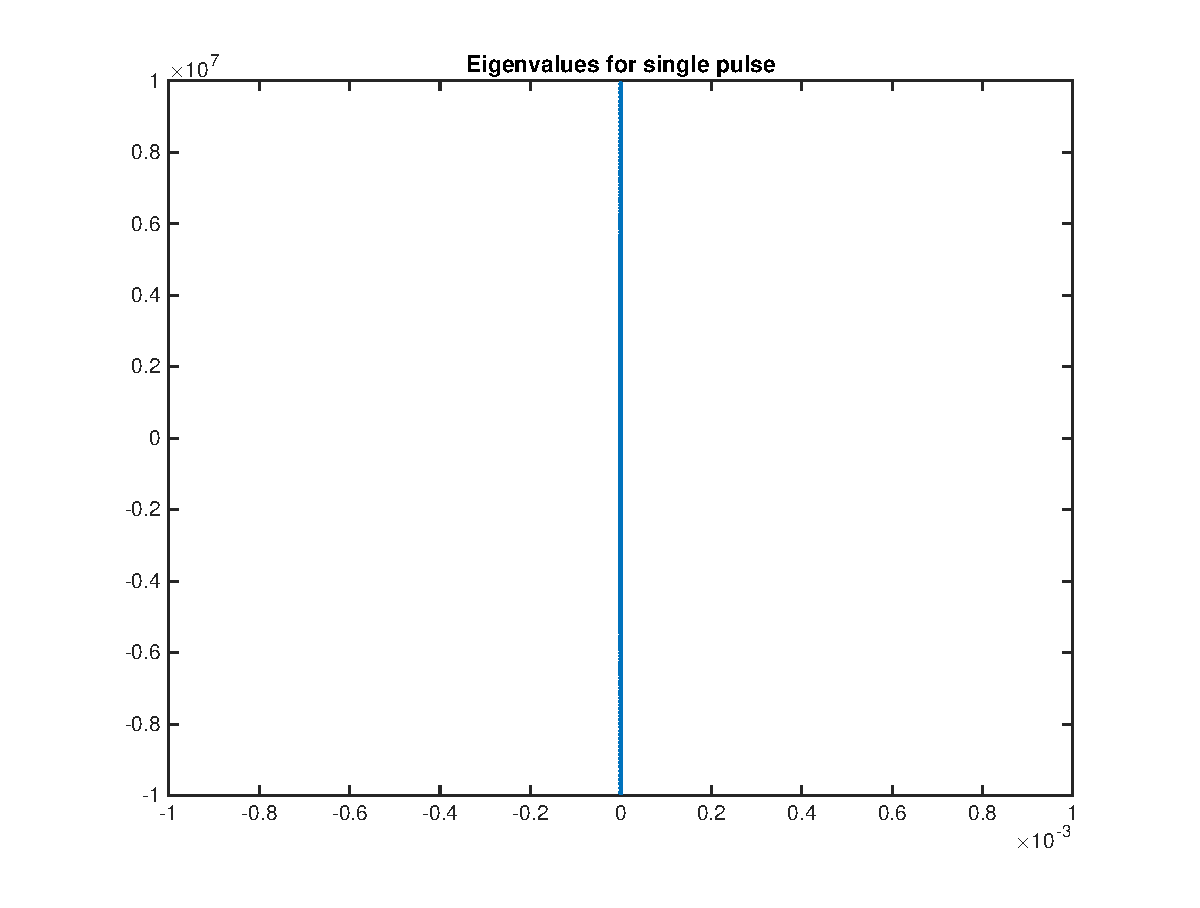
\includegraphics[width=8.5cm]{KdVsingleeig.eps}
	\end{figure}

	\item Double pulse 0: joined between origin and 1st min
	\begin{figure}[H]
	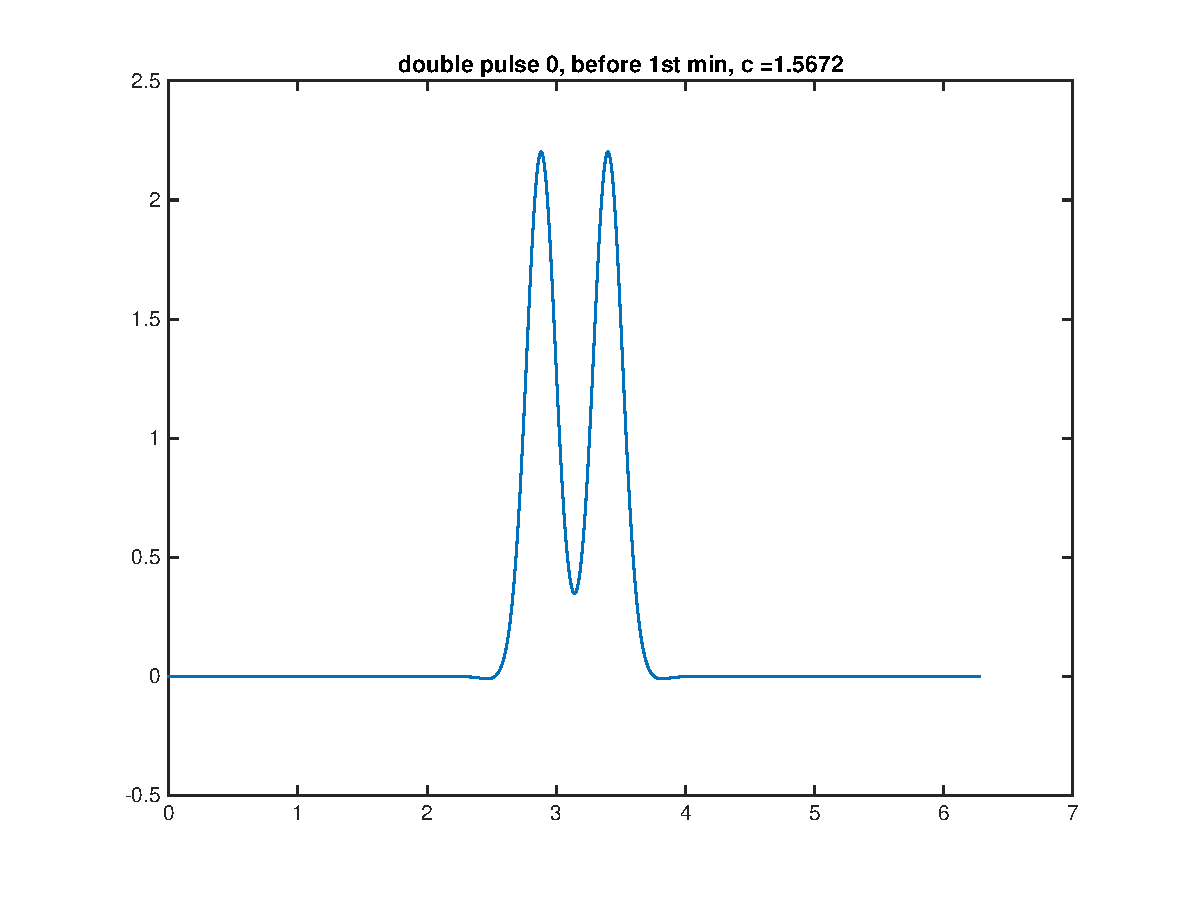
\includegraphics[width=8.5cm]{KdVdouble0.eps}
	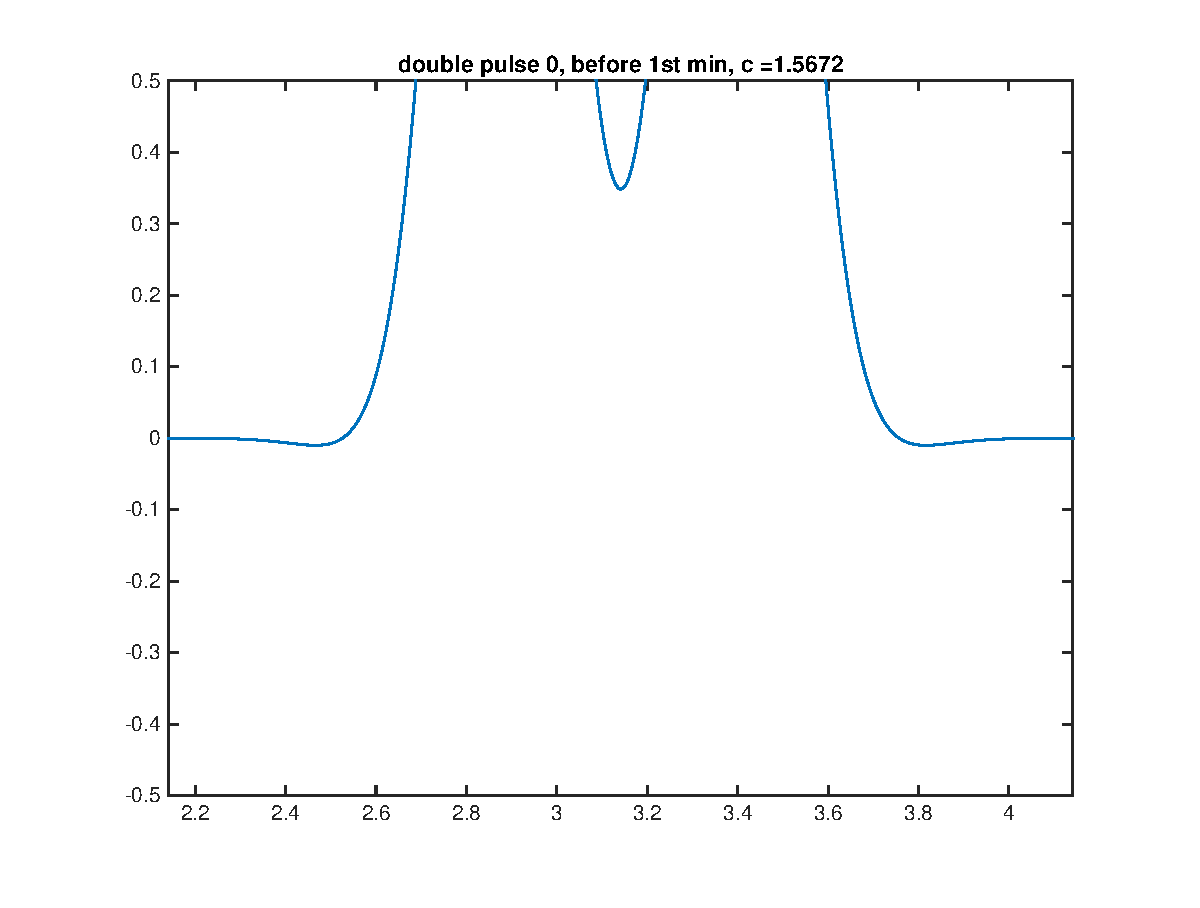
\includegraphics[width=8.5cm]{KdVdouble0zoom.eps}
	\end{figure}
	\begin{figure}[H]
	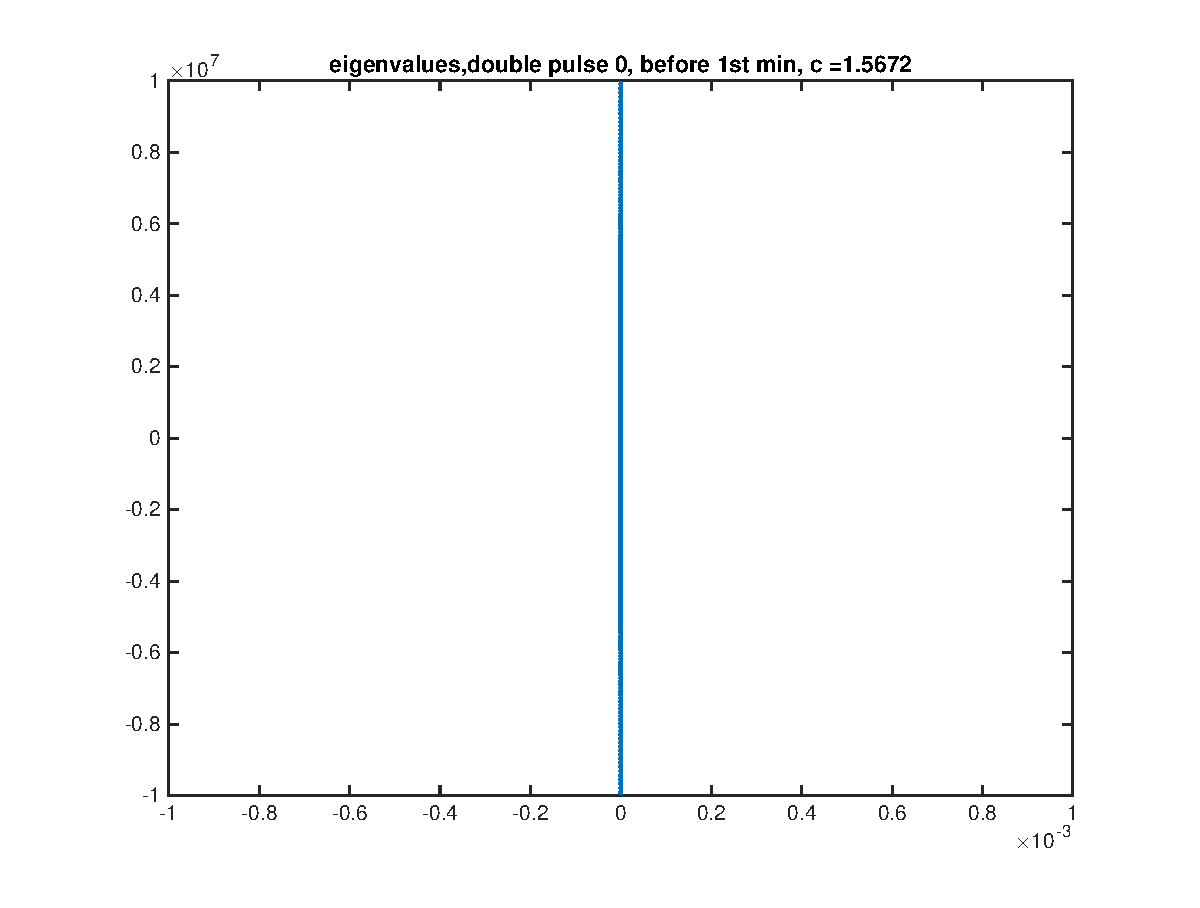
\includegraphics[width=8.5cm]{KdVdouble0eig.eps}
	\end{figure}

	\item Double pulse 1: joined at 1st min
	\begin{figure}[H]
	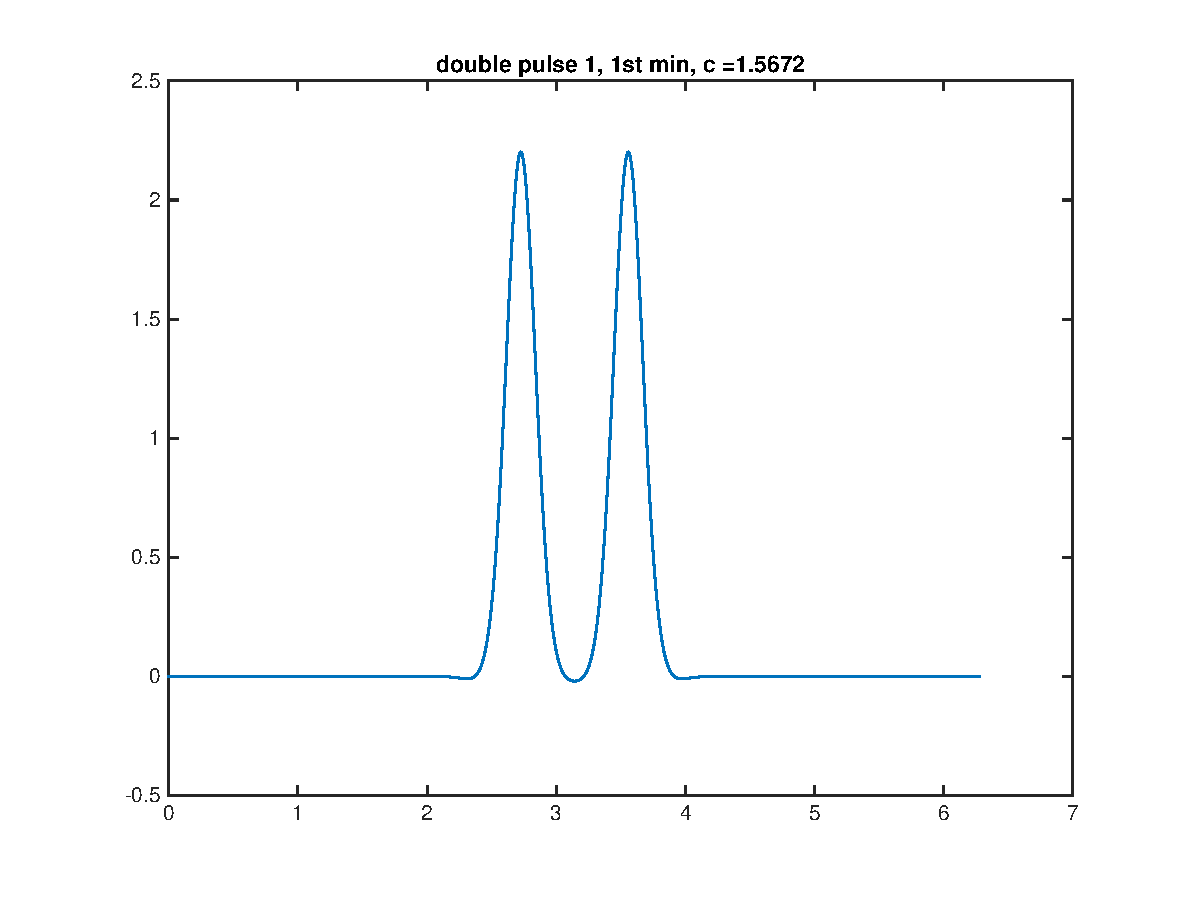
\includegraphics[width=8.5cm]{KdVdouble1.eps}
	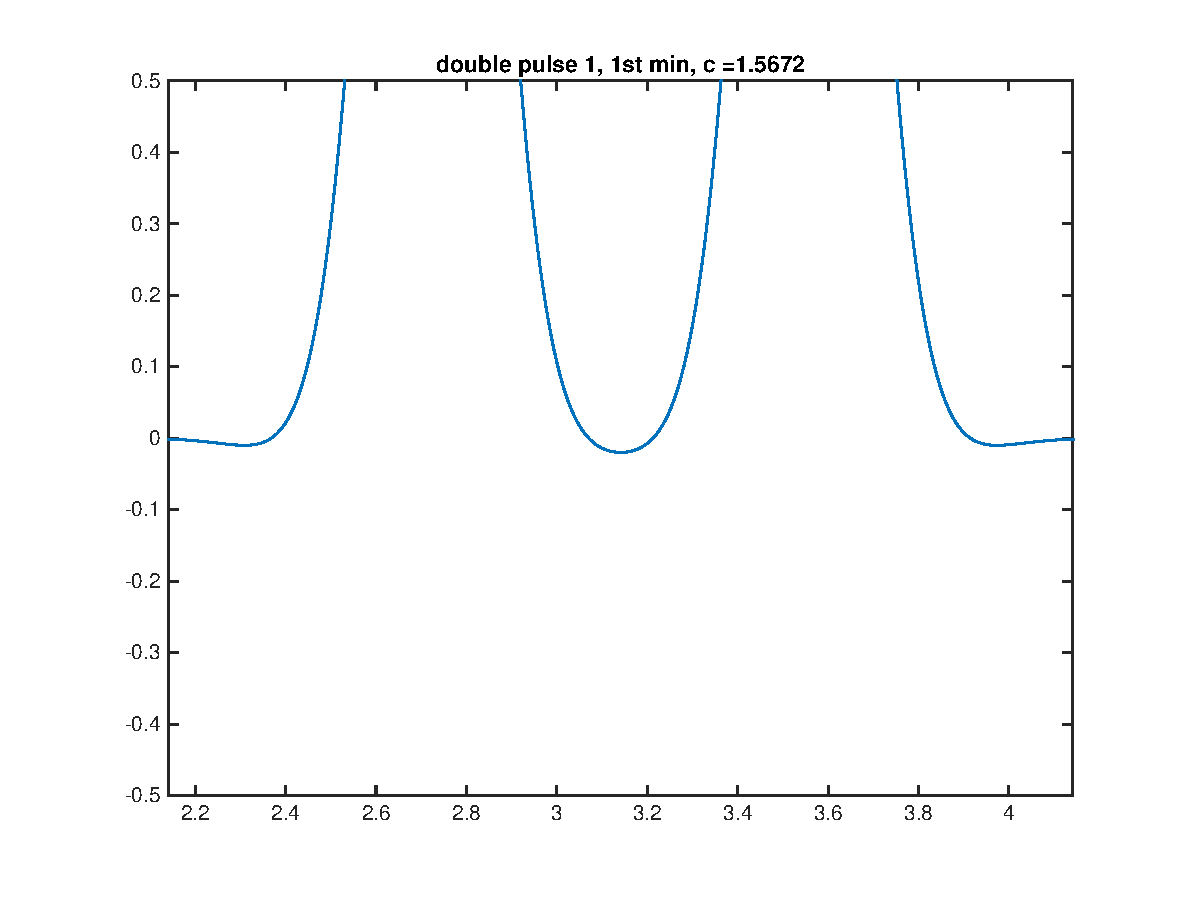
\includegraphics[width=8.5cm]{KdVdouble1zoom.eps}
	\end{figure}
	\begin{figure}[H]
	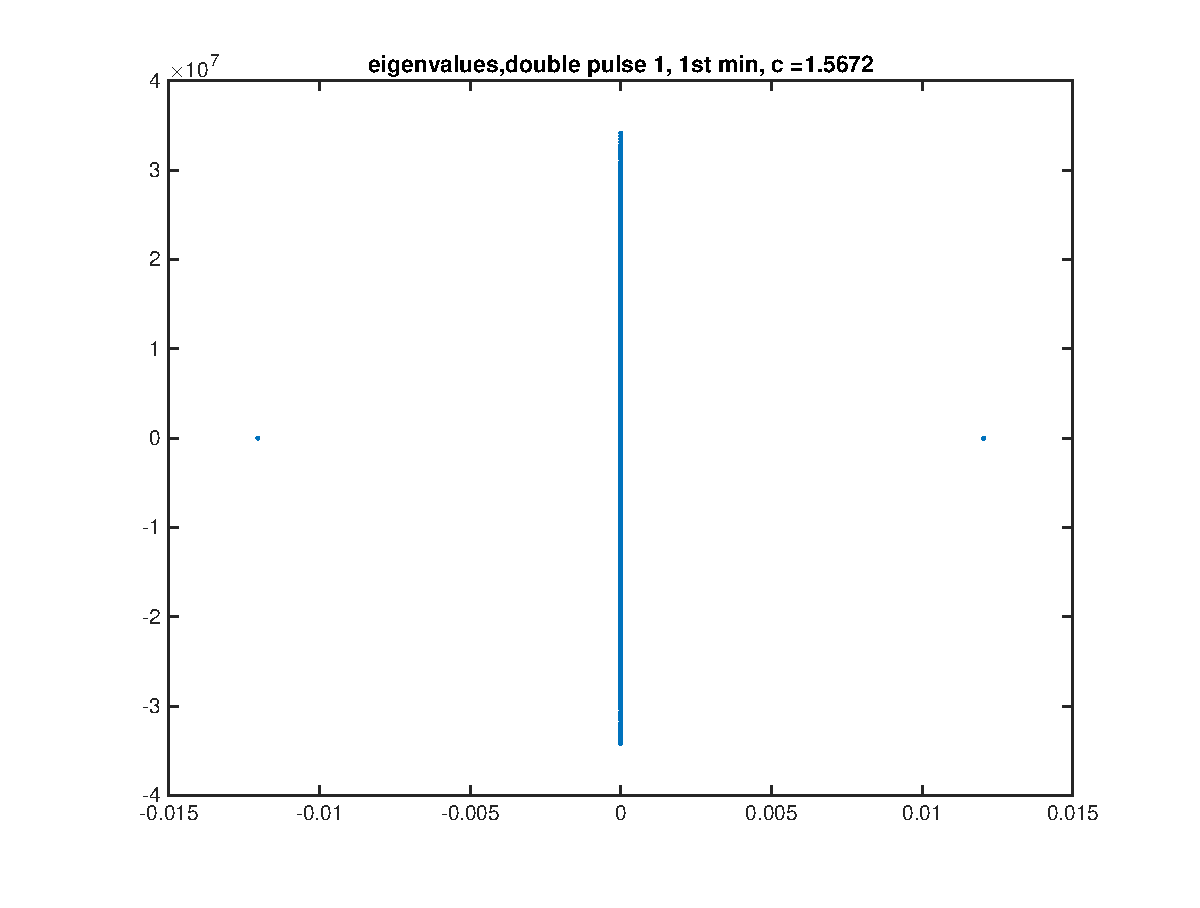
\includegraphics[width=8.5cm]{KdVdouble1eig.eps}
	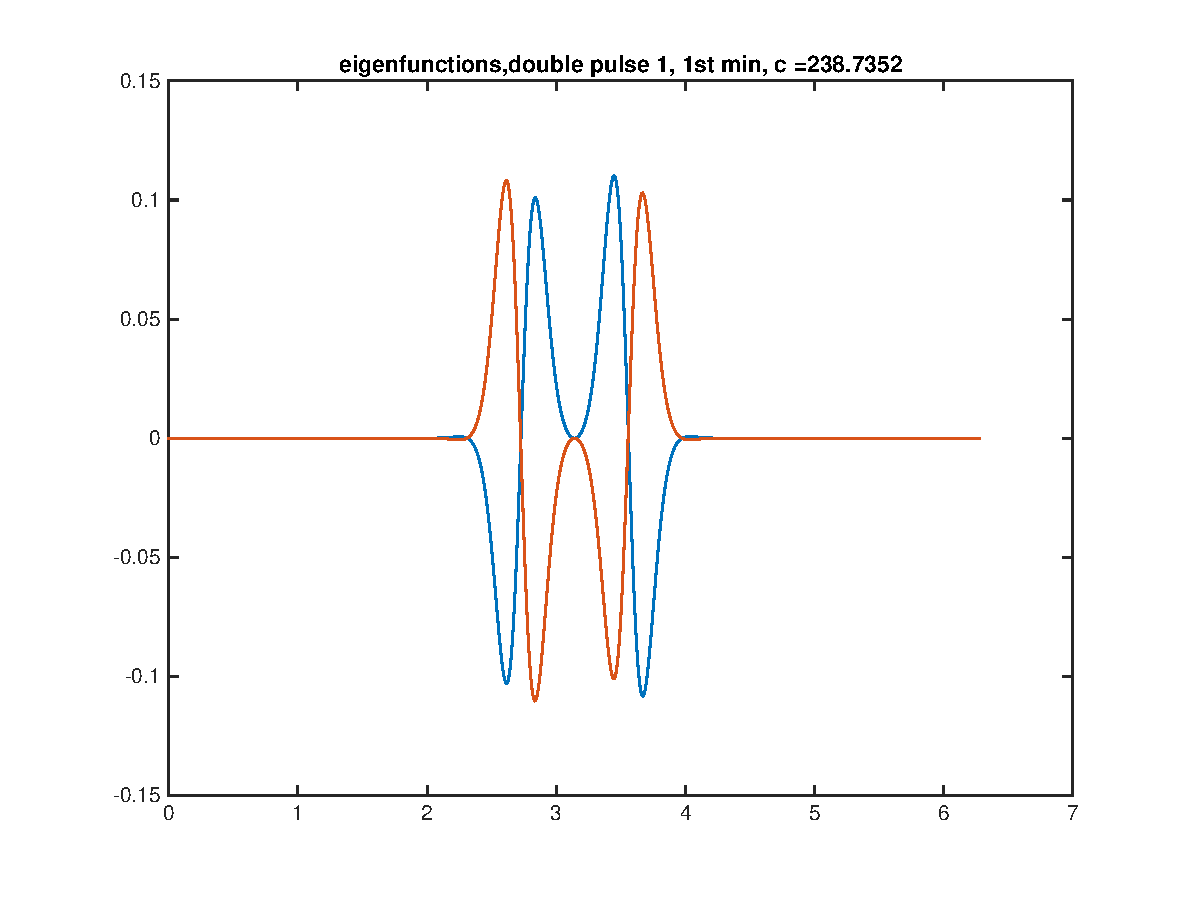
\includegraphics[width=8.5cm]{KdVdouble1eigfn.eps}
	\end{figure}

	\item Double pulse 2: joined between 1st min and 1st max
	\begin{figure}[H]
	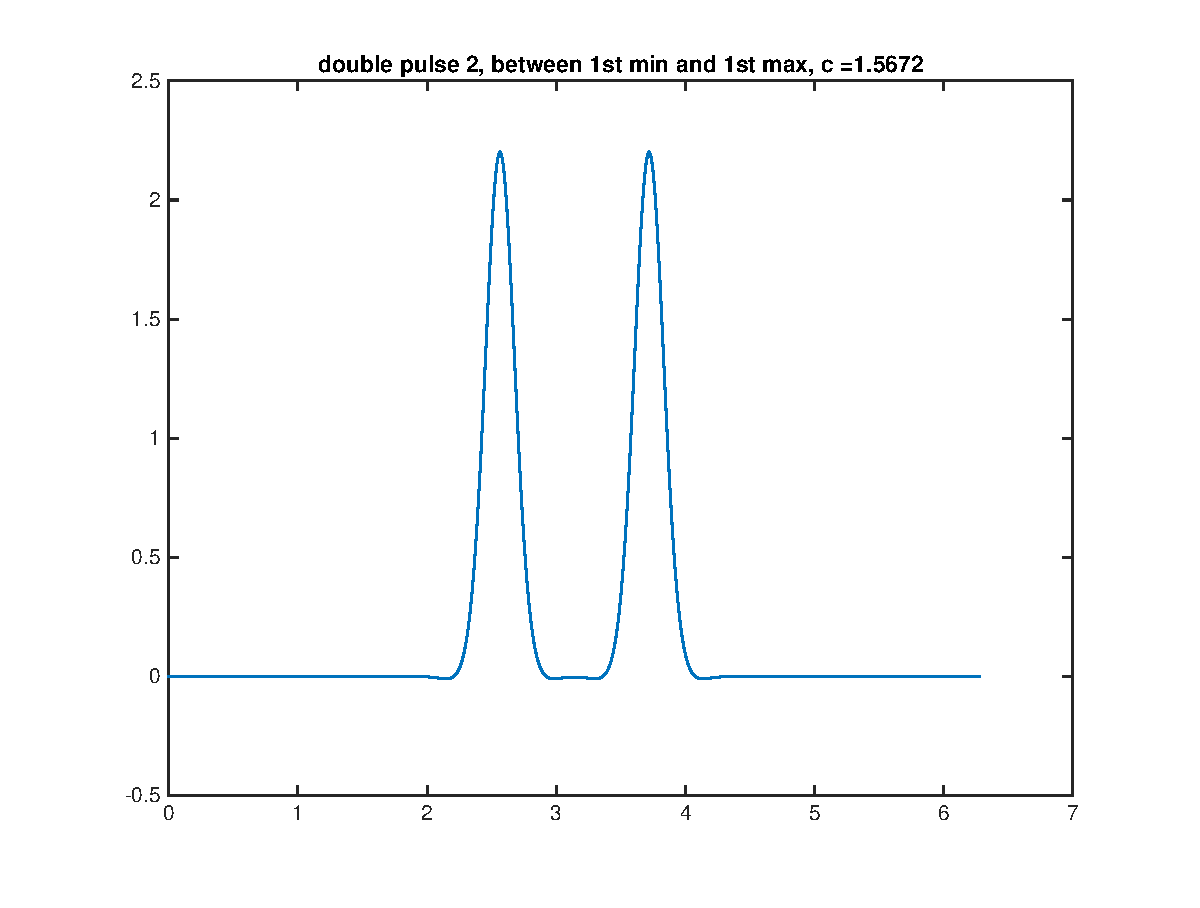
\includegraphics[width=8.5cm]{KdVdouble2.eps}
	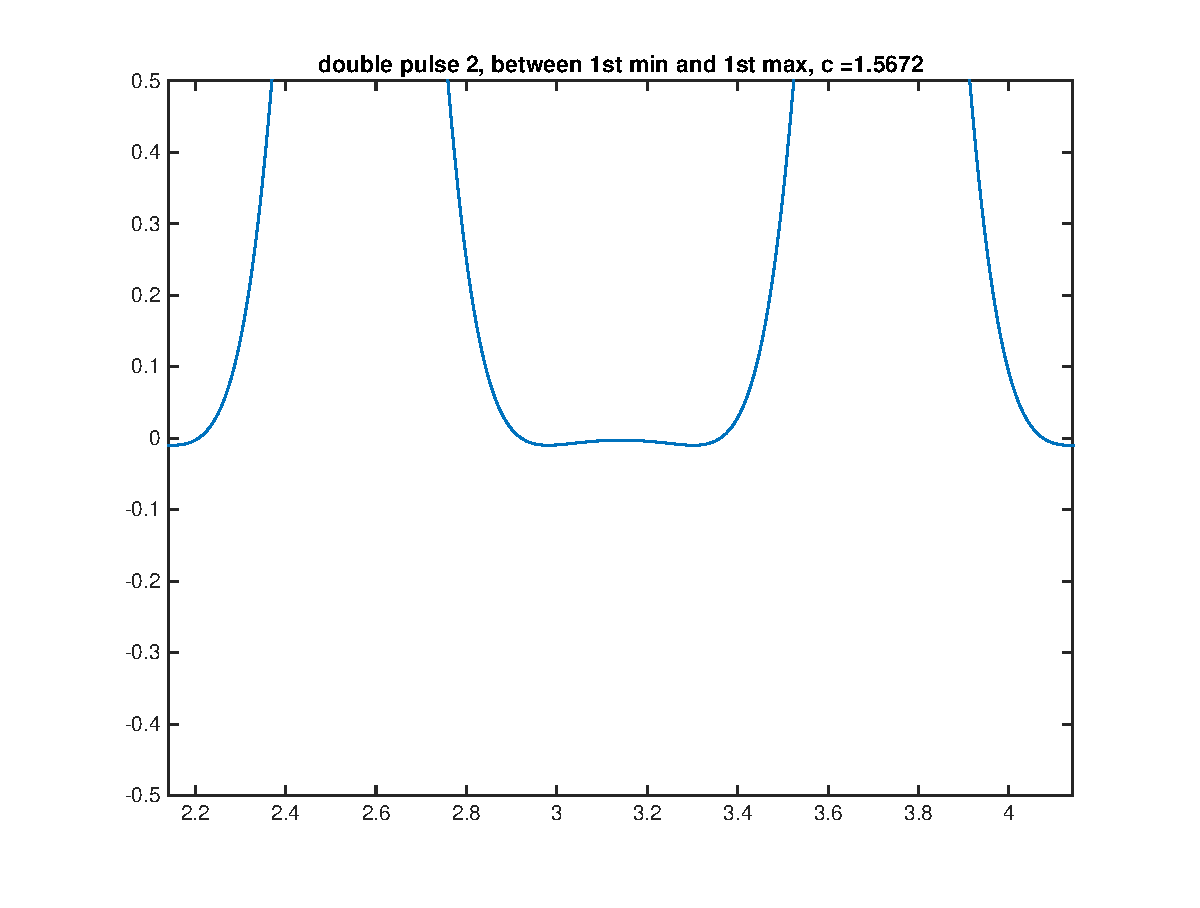
\includegraphics[width=8.5cm]{KdVdouble2zoom.eps}
	\end{figure}
	\begin{figure}[H]
	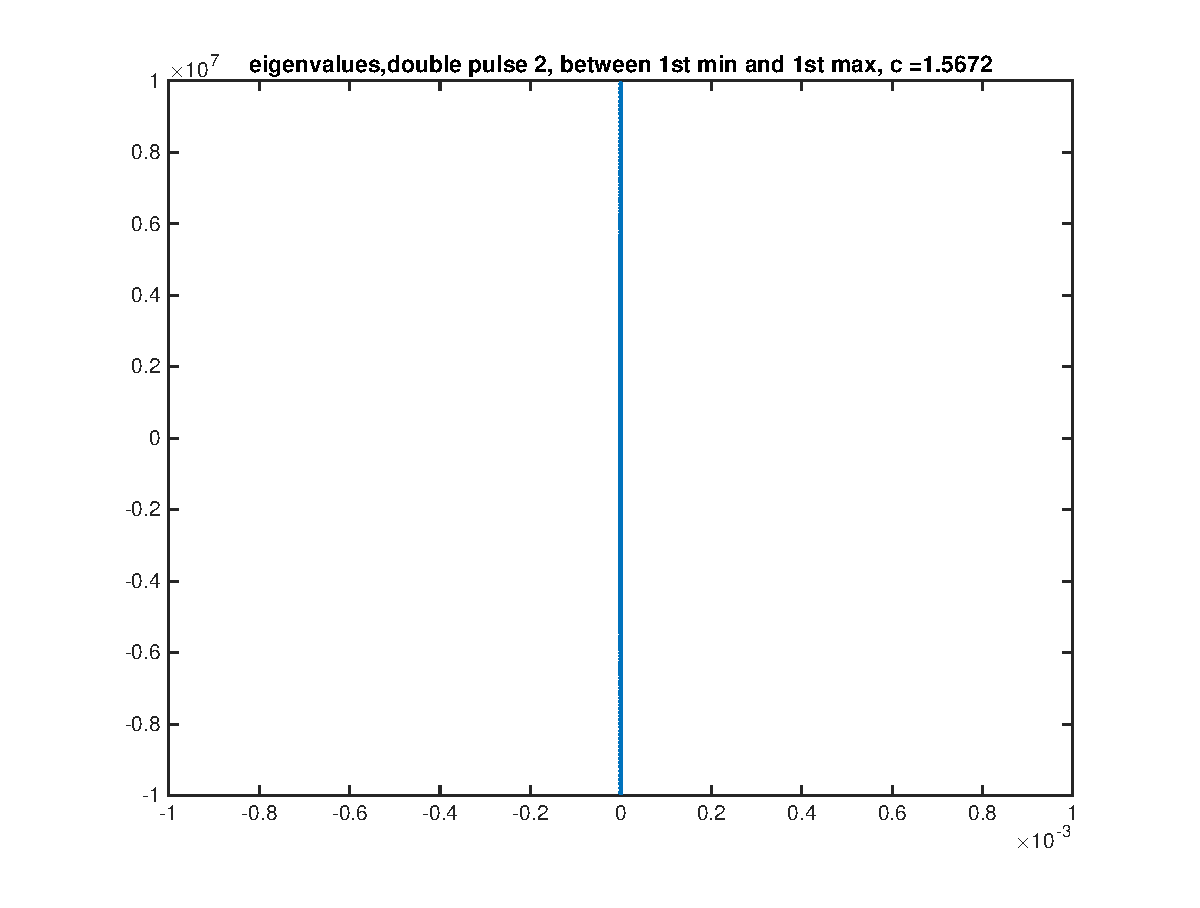
\includegraphics[width=8.5cm]{KdVdouble2eig.eps}
	\end{figure}
\end{enumerate}

A similar table to above shows the eigenvalues of the integrated operator.
\begin{figure}[H]
\begin{tabular}{ll|ll|ll}
Pulse  &         & Eigenvalue near 0  & Paired eigenvalue & Other eigenvalue  & Paired eigenvalue \\ \hline
Single &         & 5.6835e-12         &                   & -1.8484	          &                   \\
D0     & between & -1.1378e-09        & -0.0592           & -1.8561           & -1.8494           \\
D1     & min     & -1.1279e-09        & 4.8678e-04        & -1.8483           & -1.8483       \\
D2     & between & -3.0600e-12        & -4.0249e-06       & -1.8484           & -1.8484       \\
\end{tabular}
\end{figure}
As above, the paired eigenvalue near 0 flips sides appropriately. All other observations carry over.

\end{document}

